\documentclass[11pt]{article}

\usepackage{blindtext}
\usepackage{fullpage}
\usepackage{rotating}   
\usepackage{amsmath}
\usepackage{amssymb}
\usepackage{amsthm}
\usepackage{fancyhdr}
\usepackage{algorithm}
\usepackage{bm}
\usepackage{listings}
\usepackage{graphicx}
\usepackage{caption2}
\usepackage{subfigure}
\usepackage{float}
\usepackage{extpfeil}
\usepackage{color}
\usepackage{indentfirst} 
\usepackage[stable]{footmisc}
\usepackage[usenames,dvipsnames]{xcolor}
\usepackage[noend]{algpseudocode}

\newtheorem{theorem}{Theorem}[section]
\newtheorem{lemma}[theorem]{Lemma}
\newtheorem{corollary}[theorem]{Corollary}
\newtheorem{proposition}[theorem]{Proposition}
\newtheorem{definition}[theorem]{Definition}
\newtheorem{conjecture}[theorem]{Conjecture}
\newtheorem{remark}[subsection]{Remark}

%%
\newcommand\numberthis{\addtocounter{equation}{1}\tag{\theequation}}

%% define new symbols
\def\bx{\bm{x}}
\def\bb{\bm{b}}
\def\ba{\bm{a}}
\def\bc{\bm{c}}
\def\bf{\bm{f}}
\def\by{\bm{y}}
\def\bu{\bm{u}}
\def\bv{\bm{v}}
\def\BW{\bm{W}}
\def\BA{\bm{A}}
\def\bz{\bm{z}}
\def\BZ{\bm{Z}}
\def\BH{\bm{H}}
\def\BL{\bm{L}}
\def\BU{\bm{U}}
\def\BV{\bm{V}}
\def\BB{\bm{B}}
\def\BC{\bm{C}}
\def\BD{\bm{D}}
\def\BE{\bm{E}}
\def\BW{\bm{W}}
\def\BQ{\bm{Q}}
\def\BG{\bm{G}}
\def\BA{\bm{A}}
\def\BX{\bm{X}}
\def\BY{\bm{Y}}
\def\BQ{\bm{Q}}
\def\BI{\bm{I}}
\def\BR{\bm{R}}

%% define new brackets
\def\la{\left\langle}
\def\ra{\right\rangle}
\def\ln{\left\|}
\def\rn{\right\|}
\def\lb{\left(}
\def\rb{\right)}
\def\lsb{\left[}
\def\rsb{\right]}
\def\lcb{\left\{}
\def\rcb{\right\}}

%%
\DeclareMathOperator*{\argmin}{arg\,min}
\DeclareMathOperator*{\argmax}{arg\,max}

%%
\title{A Brief Insight into Complex Polynomial Root-finding and Fractals}
\author{Name: Shao Yanjun, Number: 19307110036}

\setlength{\parindent}{1em}

\begin{document}
\maketitle

%------------------------------------
\begin{abstract}
This is Daniel's final project of  "Numerical Algorithms with Case Studies II".
\end{abstract}
%-------------------------------------
%=====================
\section{Julia Set, Mandelbrot Set and Newton Fractals \footnote{Mahanta, Arun \& Sarmah, Hemanta \& Paul, Ranu \& Choudhury, Gautam. (2016). Julia set and some of its properties. 5. 99-124. }} 
The modern day interest in Julia sets and related mathematics began in the year 1920, which was initiated by French mathematician Gaston Julia. In 1918 he wrote a paper titled \textit{"M´emoire sur l’iteration des functions rationelles"}\footnote{Julia G.," M'emoire Sur I'iteration des fonctions rationelles" Journal de Math. Pure ET Appl. 8(1918) 47-	245.Republished in Herve M. (ed), Oeuvers de Gaston Julia: Vol.1, Gauthiers-Villars 1968, 121-333.
} (A Note on the Iteration of Rational Functions) where he first introduced the modern idea of a Julia set. Personally, I began my research on this topic when I was watching Numberphile videos on Youtube \footnote{\textit{https://www.youtube.com/watch?v=oCkQ7WK7vuY}}. Comments suggested that the algorithm is not too complicated to implement in Matlab, so I spent a whole afternoon to make it work with animation and relatively high resolution. Hopefully, it works quite well under finite iterations of calculation.
 
A mapping of the form reading, 
\begin{align*}
	f: z\rightarrow z^2+c\qquad c\in\mathbb{C}, |c|\le2
\end{align*}
is defined, so that for different values of the parameter $c$, we can find a
conceptually easiest way to define Julia set.
\begin{definition}
Let c be any complex number. The smallest closed set in the complex plane that contains all fixed points and all periodic points of the map $f_c(z)=z^2+c$ is called Julia set of the map $f_c$, denoted by $J_c$.
\end{definition}

We can also derive a trivial but exciting Lemma for the property of Julia Set. However, I will focus more on the visualization of it instead of paying too much attention on theoretical proof.
\begin{lemma}
	The Julia set $J_c$ of a function $f_c(z)=z^2+c$ is bounded.
\end{lemma} 
\begin{proof}
	Choose $r = \max(|c|, 2+\epsilon)$ and let $|z|\ge r$,
	\begin{align*}
		|f_c(z)|&=|z^2+c|\ge |z^2|-|c| \\&\ge (r-1)|z| \ge (1+\epsilon)|z|
	\end{align*}

	With this, we will deduce $f_c^n(z)$ for all $|z|\ge r$,
	\begin{align*}
		f_c^n(z)\ge (1+\epsilon)^n|z|\rightarrow\infty
	\end{align*}

	This will give a bound for $J_c\subset B(0,r)$.
\end{proof}

This Lemma at least gives a sound guarantee that whatever we initialize our iteration on $z\in \mathbb{C}$ and $|z|<r$, a Julia Set can be plot with amazing patterns.

A animated gif is generated in ./fig/Julia.gif directory, and here are some 'one-milion-dollar' glimpses of fixed $c\in \mathbb{C}$. Every pixel in the image represents a complex number $a+bi\in\mathbb{C}$ where $(a,b)\in[-2,2]\times[-2,2]$.
\begin{figure}[H]
	\centering
	\subfigure[$c=-1$]{
		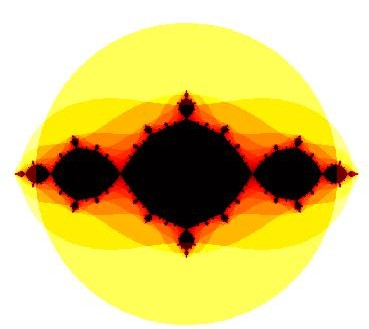
\includegraphics[width=0.2\linewidth]{Julia.jpg}
	}
	\subfigure[$c=i$]{
		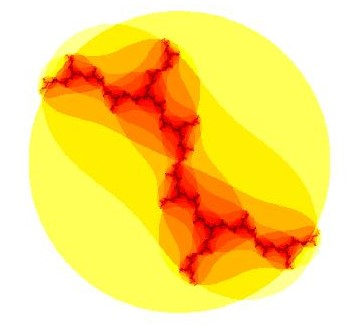
\includegraphics[width=0.2\linewidth]{Julia 2.jpg}
	}
	\subfigure[$c=-0.866 + 0.5i$]{
		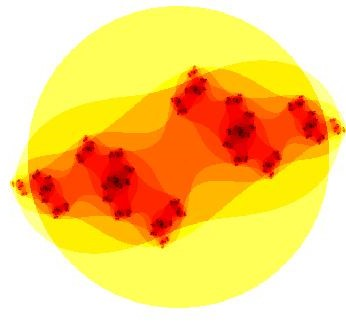
\includegraphics[width=0.2\linewidth]{Julia 4.jpg}
	}
	\subfigure[$c=0.5i$]{
	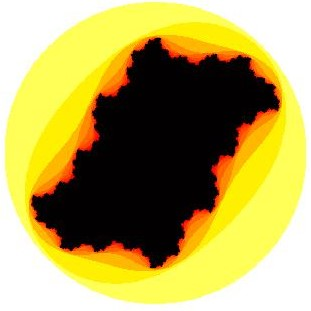
\includegraphics[width=0.2\linewidth]{Julia 3.jpg}
	}
\caption{Julia Set}
\end{figure}

Meanwhile, if we fix $z$ and represent every pixel with different $ca+bi\in\mathbb{C}$ where $(a,b)\in[-2,2]\times[-2,2]$, another fancy fractal named Mandelbrot Set can be displayed.
\begin{figure}[H]
	\centering
	\subfigure[z=0]{
		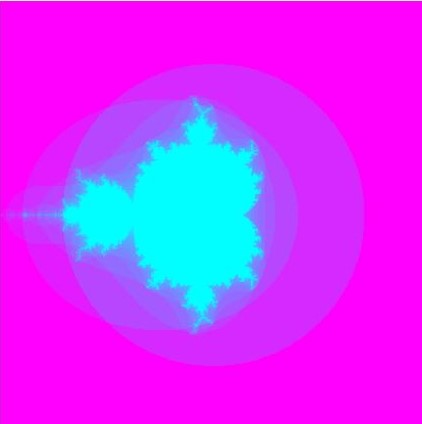
\includegraphics[width=0.3\linewidth]{Mandelbrot.jpg}
	}
	\centering
	\subfigure[z=0.5]{
		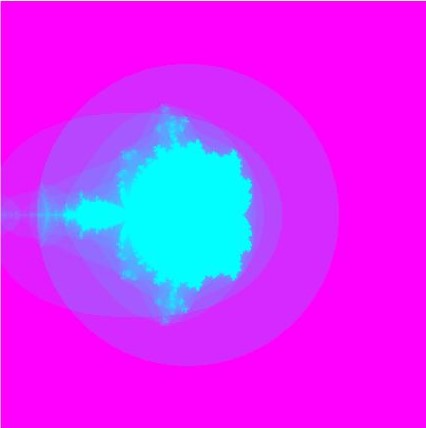
\includegraphics[width=0.3\linewidth]{Mandelbrot 2.jpg}
	}
	\subfigure[z=-0.5i (Love)]{
		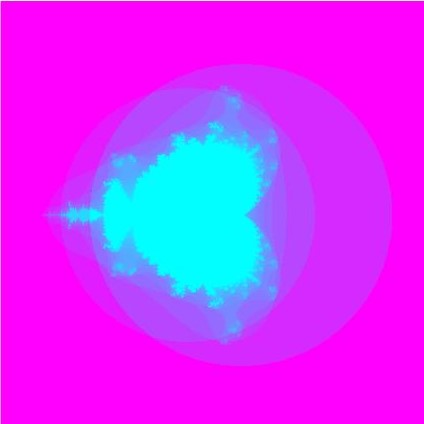
\includegraphics[width=0.3\linewidth]{Mandelbrot 3.jpg}
	}
\caption{Mandelbrot Set}
\end{figure}

However, historically, the study of iteration of maps begins with the Newton's method. Cayley and Schröder independently studied Newton's method over the complex plane during the 1870s. In 1879 paper \textit{"The Newton-Fourier Imaginary Problem"} by Sir Arthur Cayley\footnote{Peitgen H, Jurgens H., and Saupe D., "Chaos and Fractals: New Frontiers of Science" Springer Verlag, 1992.}, he applied the Newton-Fourier iterative method (also known as the Newton–Raphson method) to find the roots of the equation $f(z)=z^3+c=0$. We can also plot out the Newton Fractals of different polynomial equations, which denotes the convergence regions of the initial points $x_0\in\mathbb{C}$ to different roots on complex Plane.

The iteration rule simply reads,
\begin{align*}
	f: x_{k+1}\leftarrow x_k-\frac{P(x_k)}{P'(x_k)}
\end{align*}

Surprisingly, the convergence regions are not distinctly separated on the complex plane. There are crosses, twists and intersections between the convergence boundaries of each root.

\begin{figure}[H]
	\centering
	\subfigure[$x^3-1=0$]{
		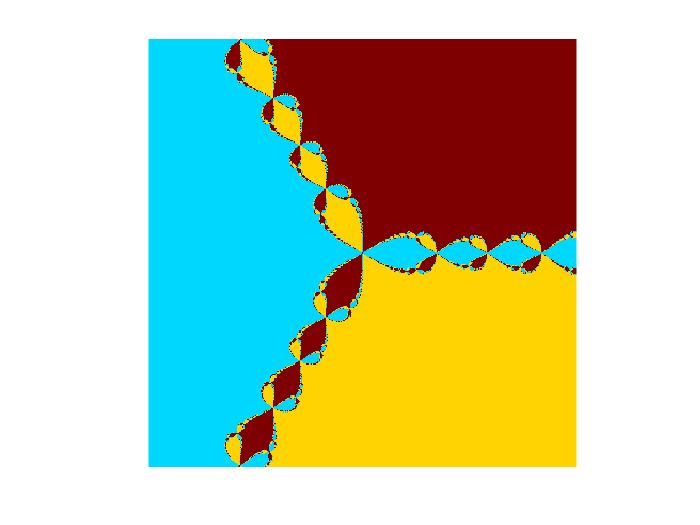
\includegraphics[width=0.35\linewidth]{Newton Fractal 3.jpg}
	}
	\centering
	\subfigure[$x^4-1=0$]{
		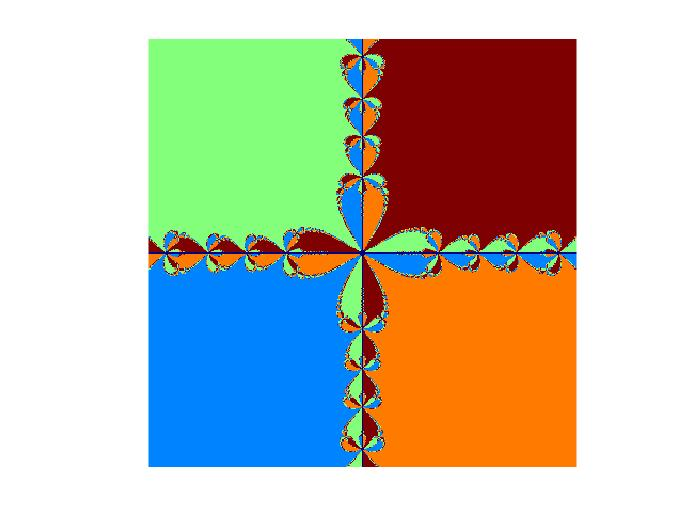
\includegraphics[width=0.35\linewidth]{Newton Fractal 4.jpg}
	}
	\subfigure[$x^5-1=0$]{
		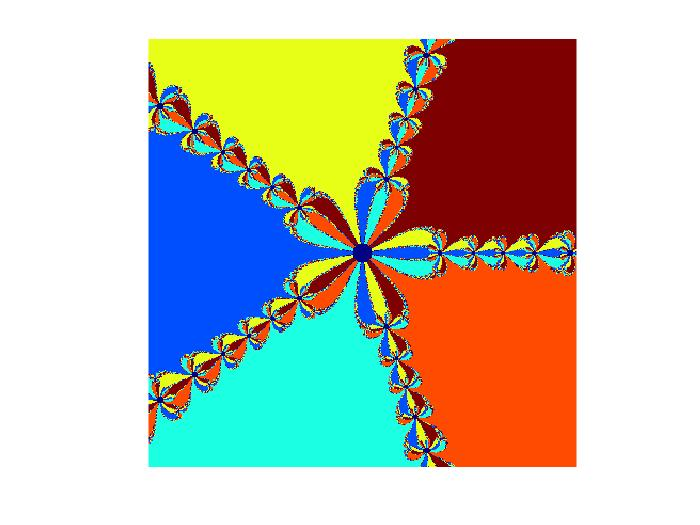
\includegraphics[width=0.35\linewidth]{Newton Fractal 5.jpg}
	}
	\subfigure[$x^{12}-1=0$]{
		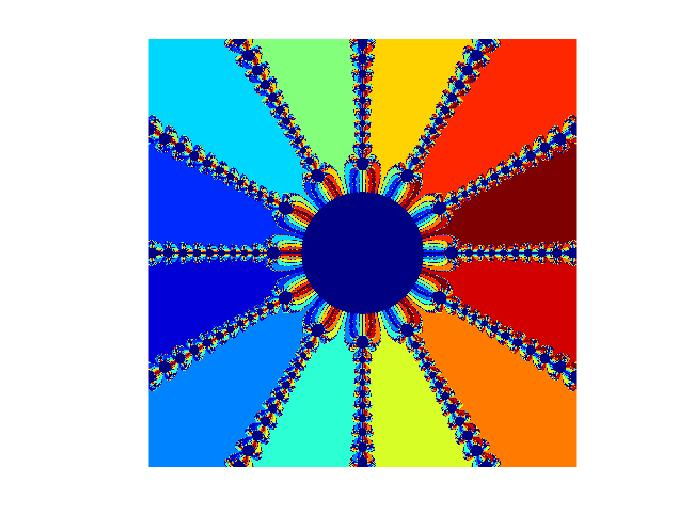
\includegraphics[width=0.35\linewidth]{Newton Fractal 12.jpg}
	}
	\caption{Newton Fractals}
\end{figure}

Intuitively, we can guess the degree of a polynomial determines the number of regions, which is trivially true because the degree of a polynomial determines the number of its roots.

\section{Newton-Raphson Method and Jenkins-Traub Method \footnote{https://en.wikipedia.org/wiki/Jenkins–Traub\_algorithm}}
Obviously, we may encounter problems with Newton-Raphson method in root-finding if the initial points are ill-chosen and fall in some unexpected regions (i.e the center blue circle of Figure 3(d)). Some global criterion for Newton-Raphson method calls into question. Otherwise, a new algorithm should be designed.

In 1968, Jenkins and Traub published a paper named \textit{"A Three-Stage Variable-Shift Iteration for Polynomial Zeros and Its Relation to Generalized Rayleigh Iteration"}\footnote{M. A. Jenkins and J. F. Traub, A three-stage variable-shift iteration for polynomial zeros in relation to generalized Rayleigh iteration, Numer. Math. 14 (1970), 252-263.} and introduced a new three-stage process for calculating the zeros of a 
polynomial with complex coefficients. I will generally introduce this algorithm and give some insights into the convergence properties. Also, what will the Fractal of this algorithm look like? It's also an interesting question to think about.

First, we will clarify some basic definitions,
\begin{definition}
	Consider polynomial $P(z)=\prod_{j=1}^{k}(z-a_j)^{m_j}\in\mathbb{C}[x]$, and its derivative will be $P'(z)=\sum_{j=1}^{k}(m_jP_j(z))$, where $P_j=P(z)/(z-a_j)$.
\end{definition}
\begin{definition}
	Define a serie of auxiliary polynomials $\{H^{(\lambda)}(z)|\lambda\in\mathbb{N}\}$, which satisfies
	\begin{align*}
		H^{(0)}(z)=P'(z)
	\end{align*}
	and
	\begin{align*}
		H^{(\lambda+1)}(z)=\dfrac{1}{z-s_\lambda}[H^{(\lambda)}(z)-\frac{H^{(\lambda)}(s_\lambda)}{P(s_\lambda)}H^{(\lambda)}(z)]
	\end{align*}
\end{definition}
And now we can show the general algorithm of Jenkins-Traub
\begin{algorithm}[H]
	\caption{Jenkins-Traub}
	\begin{algorithmic}[1]
		\Procedure{Phase 1: No-shift process}{}
			\State $H^{(0)}(z)\leftarrow P'(z)$
			\For{$\lambda=1,2,\cdots,M-1$} \Comment{M=5 is empirically good.}
			\State $H^{(\lambda+1)}(z)\leftarrow\dfrac{1}{z}[H^{(\lambda)}(z)-\dfrac{H^{(\lambda)}(0)}{P(0)}H^{(\lambda)}(z)]$
			\EndFor
		\EndProcedure
		\Procedure{Phase 2: Fixed-shift process}{}
		\State Find a fixed random $s$, $s.t.$ $|s|\le\min_{1\le i\le n}(|a_i|)$.
		\State And this will converge to the closest root $|s-a_i|\le|s-a_j| \forall 1\le j\le n$.
		\For{$\lambda=M,M+1,\cdots,L-1$}  \Comment{L is a sufficiently large number.}
		\State $H^{(\lambda+1)}(z)\leftarrow \dfrac{1}{z-s}[H^{(\lambda)}(z)-\dfrac{H^{(\lambda)}(s)}{P(s)}H^{(\lambda)}(z)]$
		\EndFor
		\EndProcedure
		\Procedure{Phase 3: Variable-shift process}{}
		\Repeat
		\State $H^{(\lambda+1)}(z)\leftarrow \dfrac{1}{z-s_\lambda}[H^{(\lambda)}(z)-\dfrac{H^{(\lambda)}(s_\lambda)}{P(s_\lambda)}H^{(\lambda)}(z)]$
		\State $s_{\lambda+1}\leftarrow s_\lambda-\dfrac{P(s_\lambda)}{\overline{H^{(\lambda+1)}}(s_\lambda)}$
		\Until{$|P(s_{\lambda+1})|\le \epsilon$}
		\EndProcedure
	\Return $s_{\lambda+1}$
	\end{algorithmic}
\end{algorithm}

And $s_{\lambda+1}$ will be an arbitrary complex root dependent on the choice of our fixed shift $s$. Continue to factorize $(z-s_{\lambda+1})$ from $P(z)$ to get $P_{k-1}(z)=P_{k}(z)/(z-s_{\lambda+1})$. Repeat Jenkins-Traub until $deg(P)=1$ so that all roots are found. 
\begin{algorithm}[H]
	\caption{Root-Finding}
	\begin{algorithmic}[1]
		\Repeat
		\State $root_i\leftarrow$Jenkins-Traub($P_{i}(z)$)
		\State $P_{i-1}(z)\leftarrow P_{i}(z)/(z-root_i)$
		\Until{$deg(P(z))=1$}\\
	\Return $roots$
	\end{algorithmic}
\end{algorithm}

Before diving deep into convergence analysis, we may play with our new algorithm and plot out some random Fractals.
\begin{figure}[H]
	\centering
	\subfigure[A strange peanut]{
		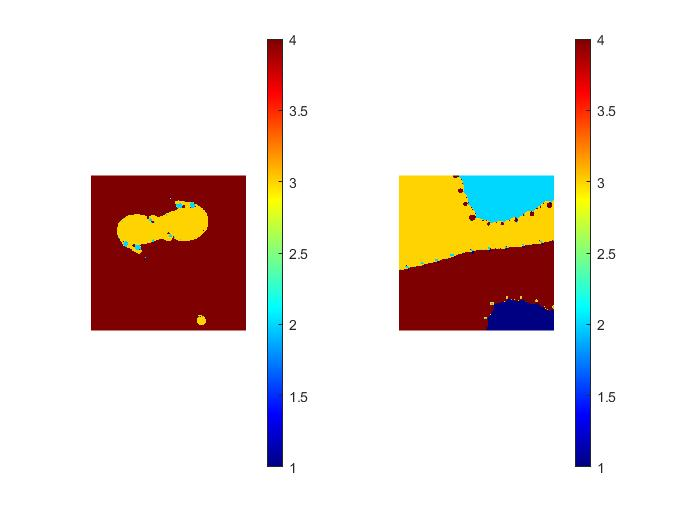
\includegraphics[width=0.45\linewidth]{Comparison2.jpg}
	}
	\centering
	\subfigure[Similar but wierd]{
		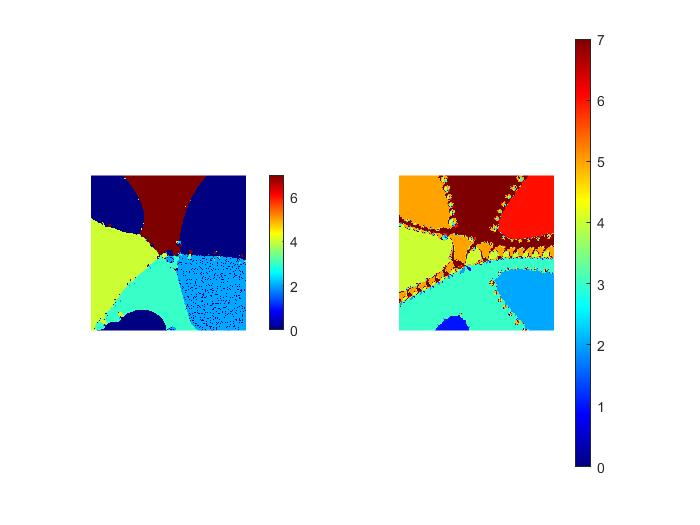
\includegraphics[width=0.45\linewidth]{Comparison3.jpg}
	}
	\subfigure[A baby sitter]{
		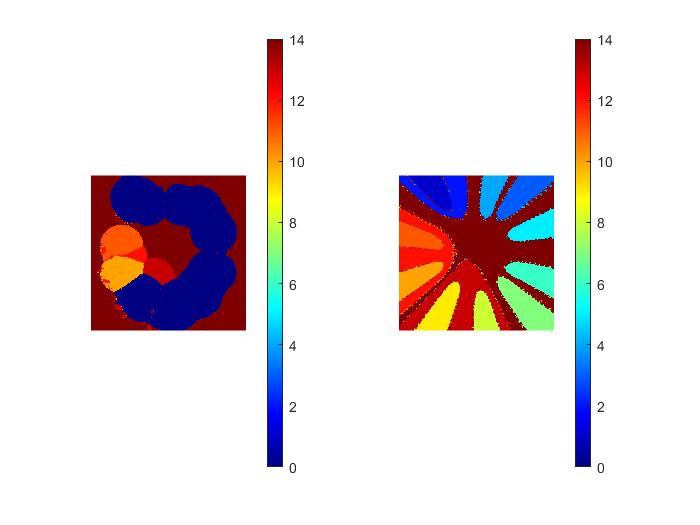
\includegraphics[width=0.45\linewidth]{Comparison4.jpg}
	}
	\subfigure[Master's painting]{
		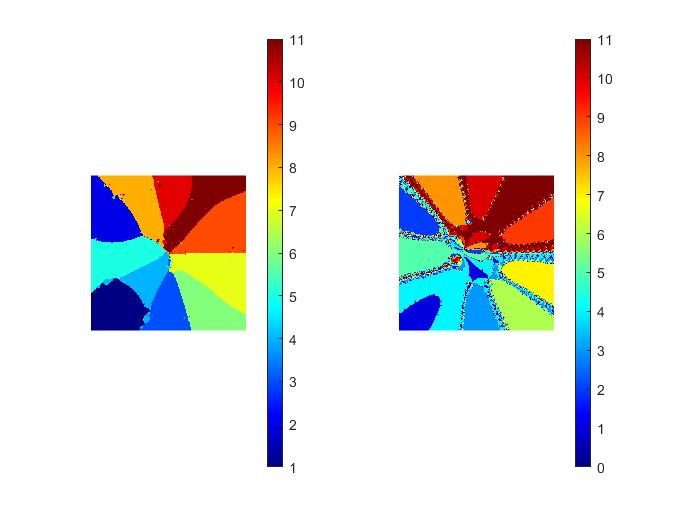
\includegraphics[width=0.45\linewidth]{Comparison5.jpg}
	}
	\caption{Newton Fractals}
\end{figure}

Most Fractals of Jenkins-Traub method look ridiculous and make no sense at all, or rather we may simply regard it as a random painting instead of Fractal.

To give an overall view of the algorithm performance, we first give some Lemma and Definitions.
\begin{lemma}
	Denote $H^{(\lambda)}(z)=\sum_{j=1}^{k}c^{(\lambda)}_jP_j(z)$, and $c^{(\lambda+1)}=\dfrac{m_j}{\prod_{t=0}^{\lambda}(s_t-a_j)}$
	\begin{proof}
		Use the iteration form,
		\begin{align*}
			H^{(\lambda+1)}(z)&=\dfrac{1}{z-s_\lambda}[H^{(\lambda)}(z)-\frac{H^{(\lambda)}(s_\lambda)}{P(s_\lambda)}H^{(\lambda)}(z)]\\
			&=\dfrac{P(z)}{z-s_\lambda}[\sum_{j=1}^{k}\dfrac{c^{(\lambda)}_j}{z-a_j}-\sum_{j=1}^{k}\dfrac{c^{(\lambda)}_j}{s_\lambda-a_j}]\\
			&=\sum_{j=1}^{k}\dfrac{c^{(\lambda)}_jP(z)}{(z-a_j)(s_\lambda-a_j)}\\
			&=\sum_{j=1}^{k}\dfrac{c^{(\lambda)}_jP_j(z)}{s_\lambda-a_j}=\sum_{j=1}^{k}c^{(\lambda+1)}_jP_j(z)
		\end{align*}
		So we have,
		\begin{align*}
			c^{(\lambda+1)}=\dfrac{c^{(\lambda)}_j}{s_\lambda-a_j}=\cdots=\dfrac{m_j}{\prod_{t=0}^{\lambda}(s_t-a_j)}
		\end{align*}
	\end{proof}
\end{lemma}
\begin{definition}
	We denote $a_1=\argmin_j(|a_j-s|)$,  $r^{(\lambda)}_j=\dfrac{s_\lambda-a_1}{s_\lambda-a_j}$, $d^{(\lambda)}_j=\dfrac{c^{(\lambda)}_j}{c^{(\lambda)}_1}$, $T_\lambda=|\dfrac{s_{\lambda+1}-a_1}{s_{\lambda}-a_1}|$.
\end{definition}
And finally here gives a simplified Theorem of convergence,
\begin{theorem}
	Given that $s$ is chosen correctly in the algorithm and $L$ is sufficiently large, if $D_L=\sum_{j=2}^{n}|d^{(L)}|< \dfrac{1}{3}$, then we will have $s_\lambda\rightarrow a_1$ when $\lambda\rightarrow\infty$
	\begin{proof}
		Since $A=\prod_{k=0}^{\lambda} T_k=\dfrac{|s_{\lambda}-a_1|}{|s_{0}-a_1|}$, if $T_\lambda<1$, $\forall\lambda\ge L$, we will have $|s_\lambda-a_1|\rightarrow0$. Next we will prove $T_\lambda<1$ using given conditions.
		\begin{align}
			\dfrac{s_{\lambda+1}-a_1}{s_{\lambda}-a_1}&=
			\dfrac{s_\lambda-\dfrac{P(s_\lambda)}{\overline{H^{(\lambda+1)}}(s_\lambda)}-a_1}{s_{\lambda}-a_1}\\
			&=1-\dfrac{P(s_\lambda)}{\overline{H^{(\lambda+1)}}(s_\lambda)(s_\lambda-a_1)}\\
			&=1-\dfrac{P(s_\lambda)\sum_{i=1}^{n}c^{(\lambda)}_j/(s_\lambda-a_j)}{P(s_\lambda)\sum_{i=1}^{n}c^{(\lambda)}_j(s_\lambda-a_1)/(s_\lambda-a_j)^2}\\
			&=1-\dfrac{1+\sum_{j=2}^{n}d^{(\lambda)}_jr^{(\lambda)}_j}{1+\sum_{j=2}^{n}d^{(\lambda)}_j[r^{(\lambda)}_j]^2}\\
			&=\dfrac{\sum_{j=2}^{n}d^{(\lambda)}_j[r^{(\lambda)}_j]^2-\sum_{j=2}^{n}d^{(\lambda)}_jr^{(\lambda)}_j}{1+\sum_{j=2}^{n}d^{(\lambda)}_j[r^{(\lambda)}_j]^2}
		\end{align}
		Since $|r^{(L)}|=|\dfrac{s_\lambda-a_1}{s_\lambda-a_j}|<1$
		\begin{align*}
			T_\lambda&<\dfrac{|\sum_{j=2}^{n}d^{(\lambda)}_j|+|\sum_{j=2}^{n}d^{(\lambda)}_j|}{1+|\sum_{j=2}^{n}d^{(\lambda)}_j|}\\&=\dfrac{2D_\lambda}{1+D_\lambda}<1
		\end{align*}
	\end{proof}
\end{theorem}

Plot out several comparison of convergence between Newton-Raphson method and Jenkins-Traub method, we can't observe as what Jenkins and Traub asserts that there method outperforms traditional Newton-Raphson method. However, they grant a convergence of any solution with polynomial degree up to infinity.
\begin{figure}[H]
	\centering
	\subfigure[]{
		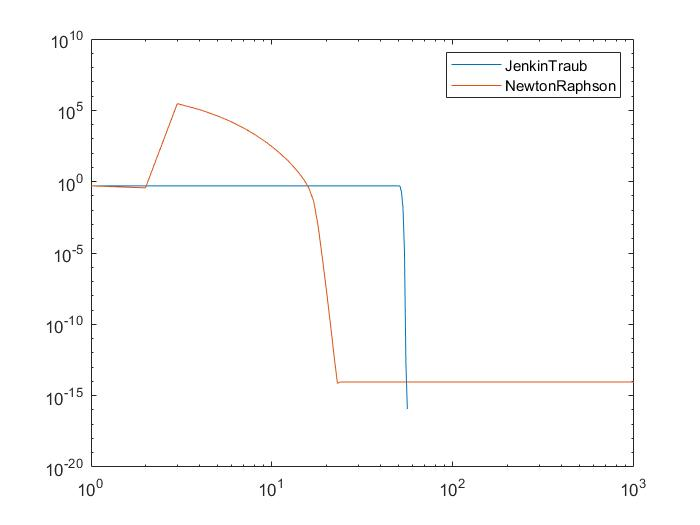
\includegraphics[width=0.33\linewidth]{Convergence3.jpg}
	}
	\centering
	\subfigure[]{
		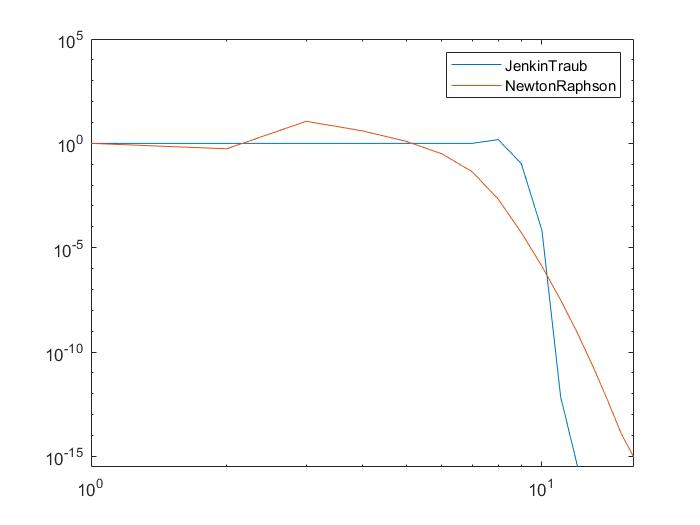
\includegraphics[width=0.33\linewidth]{Convergence4.jpg}
	}
	\subfigure[]{
		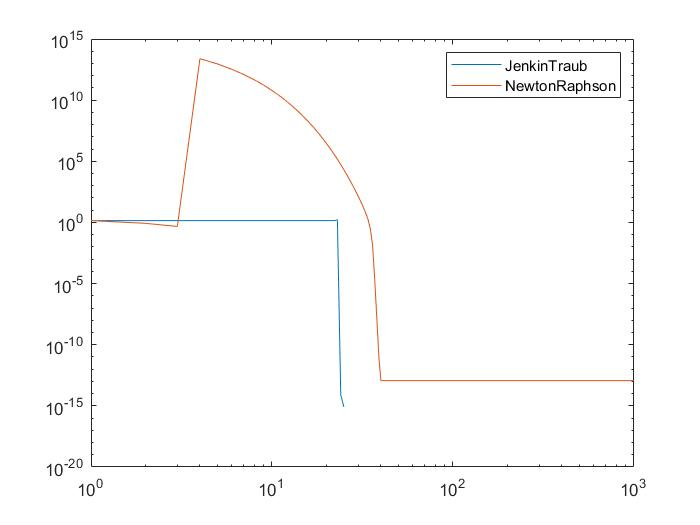
\includegraphics[width=0.33\linewidth]{Convergence1.jpg}
	}
	\subfigure[]{
		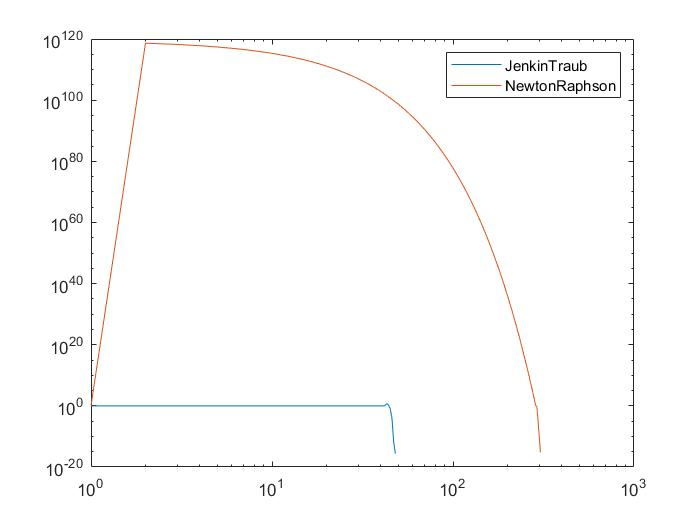
\includegraphics[width=0.33\linewidth]{Convergence7.jpg}
	}
	\caption{Convergence}
\end{figure}

This is just a glimpse of some convergence analysis. Thanks to the strong capability of Matlab to conduct complex calculations with really large numbers, we can generally observe the convergence of Newton-Raphson-method (and sometimes it outperforms Jenkins-Traub method). However, if we conduct experiment on C, which is incapable of calculations with large float numbers, Newton-Raphson method will give an error instead of finding a root.

It is worth-noted that the mathematical software Mathematica also apply this Jenkins-Traub method for calculating the zeros of a polynomial with complex coefficients. \footnote{Wankere R. Mekwi, Iterative Methods for Roots of Polynomials, Exeter College, University of Oxford, 2001.} This method, to some extent, is the state-of-art.
\section{Further Discussions and the Companion Matrix}
The above polynomial roots problem can be alternatively turned into the eigenvalues problem of the companion matrix. A polynomial equation $a_nx^n+a_{n-1}x^{n-1}+\cdots+a_1x+a_0=0$ has the following plug-in to a shifted-QR algorithm on the following matrix,
\begin{align*}
	\begin{pmatrix}
		0 & 1 &   &  &\\
		& 0 & 1 &  &\\
		&  &\ddots&\ddots\\
		&  &   &0 &1\\
		-\dfrac{a_0}{a_n} & -\dfrac{a_1}{a_n}  & \cdots & -\dfrac{a_{n-2}}{a_n}&-\dfrac{a_{n-1}}{a_n}
	\end{pmatrix}
\end{align*}

Dekker and Traub\footnote{Dekker, T. J. and Traub, J. F. (1971), The shifted QR algorithm for Hermitian matrices, Lin. Algebra Appl., 4(2), 137–154.} came up with a shifted QR algorithm for calculating the eigenvalues of the Hermitan matrices. The shifts may be viewed as Newton-Raphson iteration on a sequence of rational functions converging to a first degree polynomial. 

Also, all stages of the Jenkins–Traub complex algorithm may be represented as a linear algebra problem of determining the eigenvalues of the above companion  matrix. That is an explanation from the higher perspective, but we can easily deduce why the shift $s$ appears in the construction of $H_k(z)$. The three variants of no shift, constant shift and generalized Rayleigh shift directly matches with the three stages of the algorithm.

%-------------------------------------
%=====================
\end{document}
